\chapter{RG Flow from $\phi^4$ Theory to the 3D Ising Model}
\label{chap:3d}

\emph{Adapted from a paper currently in preparation in collaboration with 
Nikhil Anand, Emanuel Katz, Zuhair Khandker, and Matthew Walters}

\section{Introduction and Summary}

\section{Introduction}
\label{sec:Intro}

Quantum field theory, while an excellent framework for conceptualizing many of
the pressing problems in modern physics, provides little guidance in actually
calculating phenomena outside of the so-called `weakly-coupled' physical regime,
in which particles are taken to be approximately free and interactions are 
approximated via Taylor series\cite{ref:peskin}. The terms in this Taylor series
are usually represented by Feynman diagrams and grow exponentially more numerous
as orders are added in the interaction parameter; they also become more 
difficult to calculate. Accordingly, the `summing diagrams' approach to QFT is
only really useful when the interactions are weak enough that the series 
converges nicely in the first two or three orders. This is the case for many
interesting processes, including the electroweak interactions in particle 
physics, but it is also not true of many others, such as quantum chromodynamics
(QCD), which models the strong interaction.

The traditional way to investigate strongly-coupled quantum field theories like
QCD is to quantize spacetime on a lattice, thereby reducing the 
infinite-dimensional problem to a finite-dimensional one which can be simulated
on a computer\cite{ref:lattice}. This method changes the objects of study from
continuum quantum fields to a discrete set of sites -- the field can be 
reconstructed from the sites, but any variations taking place on a smaller
length scale than the lattice spacing $a$ become invisible. In the language of
QFT, this effectively places an energy cutoff at $1/a$, above which all physics
is lost.

In recent years, a competing procedure for studying strongly-coupled theories
has emerged, called Hamiltonian truncation\cite{ref:truncation}. The idea is 
that, rather than discretizing the individual modes of field excitations as a
lattice does, one will instead discretize the space of possible modes which can
be included, and then impose some natural cutoff to make this space finite. The
modes themselves are still treated as exact continuum objects, so this provides
a line of inquiry which is in some sense orthogonal to that of the lattice. 

If one is to attempt truncation, the first and paramount question is which full
basis to begin with (and subsequently truncate). Recent approaches have tended
to start with high-energy CFTs due to their orderly behavior, then add relevant
operators to the Hamiltonian and renormalize the theory to low 
energy\cite{ref:zamotrunc}. Because the spectrum of CFT operators is naturally 
discrete and bounded below in dimension $\Delta$, we can produce a finite basis 
by simply removing all operators having $\Delta > \Delta_0$ for some cutoff 
$\Delta_0$. If the CFT is placed on a sphere, this dimension cutoff corresponds 
to an energy cutoff, so by performing it we are including low-energy operators 
and excluding high-energy ones. If we then flow the theory to low energy, we 
expect that these low energy modes will be the most relevant, and therefore low 
energy phenomena ought to be represented reasonably well by 
them\cite{ref:matt3d}.

This technique has been successfully used to study QFTs in two dimensions 
\cite{ref:2d}, but a 3D formulation has not yet materialized. In this chapter,
we present a complete accounting of the theory necessary to prepare a $\phi^4$
theory for conformal truncation in 3D, along with a numerical implementation of
this truncation, which we then use to study the 3D Ising model as a proof of 
concept. We are able to observe the closing of the mass gap as the coupling 
strength is increased and correctly reproduce the spectral density of the low
energy theory.

%%%%%%%%%%%%%%%%%%%%%%%%%%%%%%%%%%%%%%%%%%%%%%%%%%%%%%%%%%%%%%%%%%%%%%%%%%%%%
%%%%%%%%%%%%%%%%%%%%%%%%%%%%%%%%%%%%%%%%%%%%%%%%%%%%%%%%%%%%%%%%%%%%%%%%%%%%%



\section{Conformal Truncation and Scalar Field Theory}
\label{sec:Model}


%%%%%%%%%%%%%%%%%%%%%%%%%%%%%%%%%%%%%%%%%%%%%%%%%%%%%%%%%%%%%%%%%%%%%%%%%%%%%


\subsection{Review of Conformal Truncation}

Conformal truncation is a method for using CFT data to numerically study the IR 
dynamics of more general QFTs. This method can be applied to any theory that can 
be described as an RG flow originating from some UV CFT deformed by one or more 
relevant operators,
\be
S = S_{\CFT} - \lambda \int d^dx \, \Ocal_R(x).
\ee
Following the approach presented in \cite{ref:matt3d}, a useful basis for the 
Hilbert space of this theory consists of UV eigenstates of the quadratic Casimir 
of the conformal group,
\be
|\Ccal,\vec{P},\mu\> \equiv \int d^dx \, e^{-iP\cdot x} \Ocal(x)|0\>,
\label{eq:basis}
\ee
where $\mu^2 \equiv P^2$. These basis states are created by primary 
operators\footnote{In this work, ``primary'' refers to any operator which is 
primary with respect to the global conformal group $SO(d,2)$ and thus 
annihilated by the special conformal generators ($\comm{K_\mu}{\Ocal(0)} = 0$). 
In 2D, this includes operators which are often referred to as ``quasi-primary'' 
or ``global primary'' in the literature.} in the original CFT, and are 
characterized by their Casimir eigenvalue, spatial momentum, and invariant mass 
(suppressing other possible quantum numbers like the spin $\ell$). 

The strategy of conformal truncation is to restrict the Hilbert space to the 
subspace spanned by states with Casimir eigenvalue $\Ccal \leq \Cmax$. The full 
Hamiltonian (CFT + deformation), when restricted to this subspace, can be 
diagonalized numerically, yielding an approximation to the true spectrum of the 
IR QFT.

To define the Hamiltonian, we first need to choose a quantization scheme. As 
discussed in \cite{ref:matt3d}, we work in lightcone quantization, with the 
Hilbert space defined on slices of constant lightcone ``time'' 
$x^+ \equiv \fr{1}{\sqrt{2}}(t+x)$. We thus need to compute matrix elements for 
the associated lightcone Hamiltonian
\be
P_+ = P_+^{(\CFT)} + \lambda \int d^{d-1}\vec{x} \, \Ocal_R(x^+=0,\vec{x}).
\ee
By construction, our basis is built from eigenstates of the CFT Hamiltonian, so 
we only need to compute matrix elements associated with the relevant 
deformation. These matrix elements are simply Fourier transforms of three-point 
functions in the original UV CFT,
\be
\<\Ccal,\vec{P},\mu| \de P_+ |\Ccal',\vec{P}',\mu'\> = \lambda \int d^d x \, d^{d-1}\vec{y} \, d^dz \, e^{i(P\cdot x - P'\cdot z)} \<\Ocal(x) \Ocal_R(y) \Ocal'(z)\>.
\label{eq:MatrixDef}
\ee
We thus only need data from the UV fixed point to study the full RG flow: the 
spectrum of local operators gives us a complete basis, while the OPE 
coefficients give us the Hamiltonian matrix elements.


%%%%%%%%%%%%%%%%%%%%%%%%%%%%%%%%%%%%%%%%%%%%%%%%%%%%%%%%%%%%%%%%%%%%%%%%%%%%%

\subsection{3D Scalar Field Theory}

Our starting point is a UV CFT of a free scalar field $\phi$ with the Lagrangian 
\begin{equation}
    \begin{aligned}
        \mathcal{L}_{\textrm{CFT}} = \frac{1}{2} : \partial_\mu \phi \partial^\mu \phi :,
    \end{aligned}
\end{equation} 
where the notation $: \mathcal{O} : $ indicates that the operator should be 
normal-ordered. We will work in $2+1$ dimensions in lightcone coordinates, which 
are defined by $x^{\pm} \equiv \frac{1}{\sqrt{2}}(t \pm x)$, as well as the 
tranverse direction $x^\bot$. The coordinate $x^+$ is treated as the ``time'' 
direction and the metric is given by 
\begin{equation}
    ds^2 = 2 dx^+ dx^- - dx^{\bot 2}.
\end{equation} 
The associated momenta are given by $p_\mu = i \partial_\mu$, from which we can 
determine the Lorentz invariant quantity 
\begin{equation}
    p^2 = 2 p_+ p_- - p_\bot^2.
\end{equation}

Our goal will be to determine the IR spectrum and eigenstates by diagonalizing 
the invariant mass-squared operator in a frame with total momentum $\vec{P}$. 
In terms of the momentum generators, this means diagonalizing 
\begin{equation}
    M^2 = 2 P_+ P_- - P_\bot^2.
\end{equation} 
We will diagonalize this operator on a basis of Casimir eigenstates associated 
with the UV free scalar. The free scalar field can be expanded in terms of its 
mode functions 
\begin{equation}
    \phi(x) = \int \frac{d^2 p}{(2\pi)^2 \sqrt{2 p_-}} \left( e^{-i p \cdot x} a_p + e^{i p \cdot x} a^\dagg_p \right),
\end{equation} 
where 
\begin{equation}
    \left[ a_p, a^\dagg_q \right] = (2\pi)^2 \delta(p-q).
\end{equation} 
This expansion for $\phi(x)$ leads to an expression for the lightcone 
Hamiltonian $P_+$ (as well as the other lightcone momenta) in terms of 
oscillator modes, as we will see momentarily. We will then diagonalize the 
mass-squared operator by similarly expressing our complete basis states in terms 
of mode functions, truncating at some maximum Casimir eigenvalue to obtain a 
finite-dimensional matrix.

After expanding in oscillator modes, the CFT Hamiltonian takes the form 
\begin{equation}
    \begin{aligned}
        P_+^{(\textrm{CFT})} = \int \frac{d^2 p}{(2\pi)^2} a^\dagg_p a_p \frac{p_\bot^2}{2p_-}.
    \end{aligned}
\end{equation}
The deformations to the UV CFT that we will study are the mass term and a 
quartic interaction, given by 
\begin{equation}
    \delta \mathcal{L} = - \frac{1}{2}m^2 \phi^2 - \frac{1}{4!} \lambda \phi^4.
\end{equation} 
This results in the following corrections to the lightcone Hamiltonian, 
respectively: 
\begin{equation}
    \begin{aligned}
        \delta P_+^{(m)} &= \int \frac{d^2 p}{(2\pi)^2} a^\dagg_p a_p \frac{m^2}{2p_-}, \label{massdeformation}
    \end{aligned}
\end{equation} 
and 
\begin{equation}
    \begin{aligned}
        \delta P_+^{(\lambda)} = \frac{\lambda}{24} \int \frac{d^2p d^2 q d^2 k}{(2\pi)^6 \sqrt{8 p_- q_- k_-}} \left( \frac{4 a^\dagg_p a^\dagg_q a^\dagg_k a_{p+q+k}}{\sqrt{2(p_- + q_- + k_-)}} + \textrm{ h.c. } + \frac{6 a^\dagg_p a^\dagg_q a_k a_{p+q-k}}{\sqrt{2(p_- + q_- - k_-)}} \right).
    \end{aligned}
\end{equation}


%%%%%%%%%%%%%%%%%%%%%%%%%%%%%%%%%%%%%%%%%%%%%%%%%%%%%%%%%%%%%%%%%%%%%%%%%%%%%

\subsection{Conformal Basis for 3D Scalar Fields}

The conformal truncation prescription amounts to diagonalizing $M^2$ on a basis 
of Casimir eigenstates. In this section, we will explain how to construct these 
eigenstates and how the basis is modified in the presence of the mass 
deformation.

Our starting point in the UV is the free massless scalar field, and so our basis 
is comprised of primary (and descendant) operators of the free scalar. In order 
to construct these operators, we have the following building blocks 
\begin{equation}
    \phi, \quad\quad\quad \partial_+ \phi, \quad\quad\quad \partial_-\phi, \quad\quad\quad \partial_\bot\phi. \label{basisbuildingblocks}
\end{equation} 
The equations of motion imply that
$\partial_+ \phi = \frac{\partial_\bot^2}{2 \partial_-} \phi$, so we can focus 
on only the $\partial_- \phi$ and $\partial_\bot \phi$ building blocks.

The idea is to construct a basis of Casimir eigenstates from these building 
blocks. In previous work, we started with the ``all-minus'' subset of the basis, 
comprised of operators built only from $\phi$ and $\partial_-$ derivatives. 
Then, we obtained the other states by acting on the all-minus states with the 
Pauli-Lubanski operator.

Our approach in this work will be more pedestrian. We will simply start with the 
building blocks eq. \eqref{basisbuildingblocks} and construct the linear 
combinations that are primary with a brute-force algorithm. These operators take 
the form 
\begin{equation}
    \mathcal{O}(x) = \sum_{\{ m_n \}} C^{\mathcal{O}}_{\{m_n\}} \partial^{m_1} \phi(x) \partial^{m_2} \phi(x) \dotsb \partial^{m_n} \phi(x),
\end{equation} 
for some yet-to-be-determined coefficients $C^{\mathcal{O}}_{\{m_n\}}$. We can 
express these operators in momentum space by inserting a complete set of states: 
\begin{equation}
    \begin{aligned}
        | \mathcal{O} ; \vec{P}, \mu \rangle &= \frac{1}{n!} \int \frac{d^2 p_1 \dotsb d^2 p_n}{(2\pi)^{2n} 2p_{1-} \dotsb 2p_{n-}} \langle p_1, \dots, p_n | \mathcal{O} ;\vec{P}, \mu \rangle | p_1, \dots, p_n \rangle \\
        &= \frac{1}{n!}\int \frac{d^2 p_1 \dotsb d^2 p_n}{(2\pi)^{2n} 2p_{1-} \dotsb 2p_{n-}} (2\pi)^3 \delta^3 \left(\sum_i p_i - P \right) F_{\mathcal{O}}(p)| p_1, \dots, p_n \rangle, \label{contstatedef}
    \end{aligned}
\end{equation} 
where the wavefunction $ F_{\mathcal{O}}(p)| p_1, \dots, p_n \rangle$ is just 
given by the overlap of the operator with a Fock space state 
\begin{equation}
    F_{\mathcal{O}}(p) = \langle \mathcal{O}(0) | p_1, \dots, p_n \rangle = \sum_{\{ m_n \}} C^{\mathcal{O}}_{\{m_n\}} p_1^{m_1} \dotsb p_n^{m_n}.
\end{equation} 
We can therefore focus on determining these polynomials, which are simply the 
Fourier transforms of local operators.

In order to determine these wavefunctions, we must find the operators that are 
annihilated by the special conformal transformations $K_\mu$. As differential 
operators acting on a generic monomial $P_+^a P_-^b P_\bot^c \phi$, they take 
the form 
\begin{equation}
    \begin{aligned}
        K_- &= 2P_+ \frac{\partial^2}{\partial P_+^2} + 2 P_\bot \frac{\partial^2}{\partial P_+ \partial P_\bot} + 2\Delta_\phi \frac{\partial}{\partial P_+} + P_- \frac{\partial^2}{\partial P_\bot^2}, \\
        K_\bot &= -2P_+ \frac{\partial^2}{\partial P_+ \partial P_\bot} - 2P_-\frac{\partial^2}{\partial P_- \partial P_\bot} - P_\bot \frac{\partial^2}{\partial P_\bot^2} - 2\Delta_\phi \frac{\partial}{\partial P_\bot} - 2 P_\bot \frac{\partial^2}{\partial P_+ \partial P_-}, \\
        K_+ &= 2P_- \frac{\partial^2}{\partial P_-^2} + 2P_\bot \frac{\partial^2}{\partial P_- \partial P_\bot} + 2\Delta_\phi \frac{\partial}{\partial P_-} + P_+ \frac{\partial^2}{\partial P_\bot^2}.
    \end{aligned}
\end{equation} 
We could determine the primary operators by then finding the null space of these 
operators acting on the space of monomials. However, this basis of primary 
operators is actually not the final basis we are after.

To explain why, we first note that we are interested in deforming the CFT 
Hamiltonian by a mass term (and interaction terms), as given in eq. 
\eqref{massdeformation}. As reviewed in Appendix \ref{sec:ConstructingBasis}, 
the presence of this mass term results in a divergence in the mass matrix 
elements. Regulating this divergence with an $\epsilon$ prescription, we find 
some eigenstates that are lifted out of the spectrum and those that remain 
finite as $\epsilon \to 0$. The eigenstates corresponding to the finite matrix 
elements are a reshuffling of the original primary basis, such that these states 
satisfy \textit{Dirichlet} boundary conditions. Explicitly, this means operators 
which have at least one factor of $P_-$ on each particle insertion to cancel 
against the Lorentz invariant measure of the mass deformation. In momentum 
space, this corresponds to wavefunctions of the type 
\begin{equation}{}
    p_{1-} p_{2-} \dotsb p_{n-} \left( \dotsb \right),
\end{equation} 
where the second set of ellipses indicates a generic function of 
$p_{i-}$, $p_{i\bot}$, and $p_{i+}$. We will therefore introduce the following 
notation to specify a Dirichlet basis state: 
\begin{equation}
    \begin{aligned}
        | \mathcal{O}; \vec{P}, \mu \rangle = &\frac{1}{n!}\int \frac{d^2 p_1 \dotsb d^2 p_n}{(2\pi)^{2n} 2p_{1-} \dotsb 2p_{n-}} (2\pi)^3 \delta^3 \left( \sum_i p_i - P \right) \\
        &\times p_{1-} p_{2-} \dotsb p_{n-} \bar{F}_{\mathcal{O}}(p) | p_1, \dotsb, p_n \rangle,
    \end{aligned}
\end{equation} 
where $\bar{F}_{\mathcal{O}}(p)$ indicates the Dirichlet wavefunction.

One might be tempted to create a basis for the Dirichlet states by taking a list
of all primary operators and throwing out the non-Dirichlet ones. Unfortunately,
this would be incomplete, because acting with $P_-$ can cause an operator to
become Dirichlet when it wasn't before. Therefore, we need to include both the
Dirichlet primaries and the non-primary Dirichlet operators for which acting
with $K$ produces non-Dirichlet states. But these, too, are not in general 
orthonormal, and lacking a good systematic way to identify an orthonormal 
subset of them, we opted to abandon the primaries altogether, instead writing
all possible below-cutoff Dirichlet states and finding an orthonormal subset
using the Gram-Schmidt process. Details of our implementation can be found in 
Appendices \ref{sec:ConstructingBasis} and \ref{sec:code}.

Finally, to complete the discussion on our basis states, we must note that $\mu$ 
as it appears in \eqref{contstatedef} is still a continuous parameter. It 
denotes the kinetic energy of the state i.e. its eigenvalue under $P^2$. In 
order to obtain a complete, \textit{discrete} basis, we must introduce some 
prescription to discretize over this parameter. A general way to do this is to 
integrate $\mu$ weighted by functions that carry some index 
$k \in \mathbb{Z}_{\ge 0}$: 
\begin{equation}
    \begin{aligned}
        | \mathcal{O}; \vec{P}, k \rangle = &\int d\mu^2 f(\mu) g_k(\mu) \frac{1}{n!} \int \frac{d^2 p_1 \dotsb d^2 p_n}{(2\pi)^{2n} 2p_{1-} \dotsb 2p_{n-}} (2\pi)^3 \delta^3 \left( \sum_i p_i - P \right) \\
        &\times p_{1-} p_{2-} \dotsb p_{n-} \bar{F}_{\mathcal{O}}(p) | p_1, \dotsb, p_n \rangle,
    \end{aligned}
\end{equation} 
where $f(\mu)$ is a measure that we have freedom to choose. The region of 
integration for $\mu$ is supposed to be taken from $[0, \infty)$. The reason 
that it is non-negative is that there is a Wightman prescription for the 2-pt. 
function of these operators that ensures positivity of the lightcone momenta. 
However, the integral will diverge and must be regulated. For this reason, we 
have to introduce a UV cutoff $\Lambda$. Cutting off the integral and rescaling 
the region of integration to $[0,1]$ we find that our final states are given 
by
\begin{empheq}[box=\fbox]{align}
    | \mathcal{O}; & \vec{P}, k \rangle = \frac{1}{\sqrt{2\pi} P_-^{n + |\boldsymbol{\lambda}_-|} \Lambda^{\frac{n-5}{2} + |\boldsymbol{\lambda}_\bot|}}\int_0^{1} \frac{d\bar{\mu}^2}{\bar{\mu}^{\frac{n-3}{2} + |\boldsymbol{\lambda}_\bot|}} g_k(\bar{\mu}) \label{eqn:finalbasisstates}\\
    &\times \frac{1}{n!} \int \frac{d^2 p_1 \dotsb d^2 p_n}{(2\pi)^{2n} 2p_{1-} \dotsb 2p_{n-}} (2\pi)^3 \delta^3 \left( \sum_i p_i - P \right) \\
    &\times p_{1-} p_{2-} \dotsb p_{n-} \bar{F}_{\mathcal{O}}(p) | p_1, \dotsb, p_n \rangle \nonumber, 
\end{empheq} 
where we have defined the dimensionless $\bar{\mu} \equiv \frac{\mu}{\Lambda}$ 
and $|\boldsymbol{\lambda}_{-,\bot}|$ count the number of $-$ and $\bot$ 
derivatives in $\bar{F}_{\mathcal{O}}(p)$, respectively. In this paper, we 
discretize $\mu$ into linearly spaced bins:
\begin{equation}
    \begin{aligned}
        g_k(\bar{\mu}) = \frac{1}{\sqrt{\bar{\mu}^2_k - \bar{\mu}^2_{k-1}}} \left[ \theta(\bar{\mu}^2 - \bar{\mu}^2_{k-1}) - \theta(\bar{\mu}^2 - \bar{\mu}^2_k) \right], \label{gks}
    \end{aligned}
\end{equation} 
where $\theta$ is the Heaviside step function. The purpose of the above equation 
is to the set the region of integration in $\bar{\mu}$ to be in a bin between 
$\bar{\mu}_{k-1}$ and $\bar{\mu}_k$. Truncating at some $k_{\textrm{max}}$, we 
can obtain a discrete, finite-dimensional basis of Dirichlet states. The 
normalization of these weight functions is chosen such that 
\begin{equation}
    \int_0^1 d\bar{\mu}^2 g_k(\bar{\mu}) g_{k'}(\bar{\mu}) = \delta_{k k'}.
\end{equation}

This completes our discussion of computing the Dirichlet basis. To summarize: we 
tabulate all possible monomials $P_+^a P_-^b P_\bot^c \phi$ that satisfy 
Dirichlet boundary conditions and obtain the orthonormal linear combinations 
through a Gram-Schmidt procedure. We discretize in $\mu$ using the weight 
functions in eq. \eqref{gks} and truncate at some 
$\mathcal{C}_{\textrm{max}}$, $k_{\textrm{max}}$ obtain our final discrete, 
truncated basis.


%%%%%%%%%%%%%%%%%%%%%%%%%%%%%%%%%%%%%%%%%%%%%%%%%%%%%%%%%%%%%%%%%%%%%%%%%%%%%


\subsection{Review of Spectral Densities}

After we have truncated the basis to some $\Cmax$ and computed the associated 
Hamiltonian matrix elements, we can construct the invariant mass operator
\be
M^2 = 2P_+ P_-.
\ee
Because our basis consists of $P_-$ eigenstates, diagonalizing this Lorentz 
invariant operator is actually equivalent to diagonalizing the lightcone 
Hamiltonian $P_+$.

The mass eigenvalues that result from diagonalizing $M^2$ are an approximation 
to the spectrum of the IR QFT. However, in addition to the eigenvalues, we also 
obtain the associated eigenstates $|\mu_i\>$, which we can use to compute 
dynamical IR observables. One natural and important observable for us to study 
is the spectral density of any local operator $\Ocal(x)$,
\be
\rho_\Ocal(\mu) \equiv \sum_i |\<\Ocal(0)|\mu_i\>|^2 \, \de(\mu^2 - \mu_i^2).
\label{eq:rho}
\ee
As shown in eq.~\eqref{specdef}, spectral densities encode the same 
information as real-time, infinite-volume correlation functions. For presenting 
results, it will be more convenient to show the integrated spectral density,
\be
I_\Ocal(\mu) \equiv \int_0^{\mu^2} d\mu^{\prime\,2} \, \rho_\Ocal(\mu') = \sum_{\mu_i \leq \mu} |\<\Ocal(0)|\mu_i\>|^2,
\label{eq:I}
\ee
which contains the same dynamical information as the spectral density.



%%%%%%%%%%%%%%%%%%%%%%%%%%%%%%%%%%%%%%%%%%%%%%%%%%%%%%%%%%%%%%%%%%%%%%%%%%%%%
%%%%%%%%%%%%%%%%%%%%%%%%%%%%%%%%%%%%%%%%%%%%%%%%%%%%%%%%%%%%%%%%%%%%%%%%%%%%%



\section{Sanity Checks}
\label{sec:SanityChecks}

In this section, we perform consistency checks in the free massive theory where 
$\lambda = 0$. We then compare with theoretical predictions, which gives us a 
nontrivial check of the Dirichlet basis.

In section \ref{sec:theoryspecdens}, we first explain how to compute the 
theoretical predictions for the spectral density associated with a generic local 
operator $\mathcal{O}_{\mu_1, \dots, \mu_{\ell}}(x)$. We then compare these 
analytic answers to the numerical results obtained from conformal truncation. 
We will primarily focus on comparisons involving the energy-momentum tensor.


%%%%%%%%%%%%%%%%%%%%%%%%%%%%%%%%%%%%%%%%%%%%%%%%%%%%%%%%%%%%%%%%%%%%%%%%%%%%%


\subsection{Spectral Densities in Free Field Theory} \label{sec:theoryspecdens} 
Let's briefly review some details about spectral densities of operators in free 
massive theory. The spectral density is the decomposition of the two-point 
correlation function in terms of mass eigenstates:
\begin{equation}
    \langle \mathcal{O}(x) \mathcal{O}(0) \rangle = \int d\mu^2 \rho_{\mathcal{O}}(\mu) \int \frac{d^2 P}{(2\pi)^2 2 P_0} e^{-i P \cdot x}.\label{specdef}
\end{equation}
Forbrevity, we have omitted any tensor structure, but the operators appearing on
theLHS could, for example, be various components of spinning operators. In a
freetheory, we can expand the correlator on the LHS in terms of Fock space
modes:
\begin{equation}
    \begin{aligned}
        \langle \mathcal{O}(x) \mathcal{O}(0) \rangle &= \frac{1}{n!} \int \frac{d^3 p_1 \dotsb d^3 p_n}{(2\pi)^{3n}} \prod_i (2\pi) \delta(p_i^2-m^2) | \langle \mathcal{O}(0) | p_1, \dots, p_n \rangle |^2 e^{-i \left(\sum_i p_i \right) \cdot x} \\
        &= \int \frac{d\mu^2}{2\pi} \frac{1}{n!} \int \frac{d^3 p_1 \dotsb d^3 p_n}{(2\pi)^{3n}} \left( \prod_i (2\pi) \delta(p_i^2-m^2)\right) (2\pi)^3 \delta^3 \left( P - \sum_i p_i \right) \\
        &\,\,\, \times | \langle \mathcal{O}(0) | p_1, \dots, p_n \rangle |^2 \times \int \frac{d^2 P}{(2\pi)^2 2P_0} e^{-i P \cdot x},
    \end{aligned}
\end{equation} 
where we inserted a complete set of states and used the fact that 
$d^3P = d\mu^2 \frac{d^2 P}{2P_0}$. Equating this to eq.~\eqref{specdef}, we can 
therefore obtain an explicit equation for the spectral density associated with 
any local operator $\mathcal{O}$: 
\begin{equation} 
    \rho_{\mathcal{O}}(\mu) = \frac{1}{2\pi n!} \int \frac{d^3 p_1 \dotsb d^3 p_n}{(2\pi)^{3n}} \left( \prod_i (2\pi) \delta(p_i^2 - m^2) \right) (2\pi)^3 \delta^3 ( P - \sum_i p_i ) | \langle \mathcal{O}(0) | p_1, \dots, p_n \rangle |^2. \label{specdensexplicit}
\end{equation} 
This formula also holds for operators with spin, so that we can compare 
theoretical predictions for spectral densities of various components of spinning 
operators. The simplest way to apply eq. \eqref{specdensexplicit} is to compute 
the overlap $| \langle \mathcal{O}(0) | p_1, \dots, p_n \rangle |$, evaluate the 
integrals in the total momentum frame 
$P = (\mu, \vec{0})$, $p_i = (E_i, \vec{p}_i)$, and then perform a boost to the 
lightcone frame. Let's see how this works for a few examples.

Consider the spectral density associated with the simplest two-particle operator 
$\phi^2$. The overlap of this operator with the two-particle Fock space state is 
simply 
\begin{equation}
    \langle \phi^2(0) | p_1, p_2 \rangle = 2.
\end{equation} 
Plugging this into eq. \eqref{specdensexplicit}, and evaluating in the frame 
\begin{equation}
    P = (\mu, \vec{0}), \quad\quad\quad p_1 = (E_1, \vec{p}_1), \quad\quad\quad p_2 = (E_2, \vec{p}_2),
\end{equation} 
we find 
\begin{equation}
    \rho_{\phi^2}(\mu) = \frac{1}{4\pi \mu} \theta(\mu - 2m).
\end{equation} Note that the step function signifies that the two-particle 
spectral density starts at the two-particle threshold, as expected. There is no 
need to boost this answer to the lightcone frame as this spectral density is 
associated with the scalar two-point function $\langle \phi^2 \phi^2 \rangle$. 
We can repeat this analysis for any $\phi^n$ operator which gives the spectral 
density 
\begin{equation}
    \rho_{\phi^n}(\mu) = \frac{n!(\mu-n m)^{n-2}}{(n-2)!(4\pi)^{n-1 2\mu}}.
\end{equation}

Now let's consider a more nontrival example of the stress-energy tensor. It is 
given by 
\begin{equation}
    T_{\mu\nu} = \frac{3}{4} \partial_\mu \phi \partial_\nu \phi - \frac{1}{4} \eta_{\mu\nu} \partial_{\sigma} \phi \partial^\sigma \phi - \frac{1}{4} \phi \partial_\mu \partial_\nu \phi + \frac{1}{2}m^2 \eta_{\mu\nu} \phi^2.
\end{equation} 
Let's start with the all minus component $T_{--}$. The overlap is given by 
\begin{equation}
    \langle T_{--}(0) | p_1, p_2 \rangle = - \frac{1}{4} \left(6 p_{1-} p_{2-} - p_{1-}^2 - p_{2-}^2 \right).
\end{equation} 
We can evaluate the integrals in eq. \eqref{specdensexplicit} by noting that 
\begin{equation}
    p_{1 \pm} = \frac{1}{\sqrt{2}} (E_1 \pm p_{1x}), \quad\quad\quad p_{2 \pm} = \frac{1}{\sqrt{2}}(E_2 \pm p_{2,x}),
\end{equation} 
which gives 
\begin{equation}
    \tilde{\rho}_{T_{--}}(\mu) = \frac{\mu^4 - 8 \mu^2 m^2 + 48 m^4}{2048 \pi \mu},
\end{equation} 
where the tilde indicates that we still need to boost to the lightcone frame. We 
have computed the spectral density associated with $T_{--}$ in the frame 
$(P_+, P_-, P_\bot) =\left( \frac{\mu}{\sqrt{2}}, \frac{\mu}{\sqrt{2}}, 0 \right)$ 
while the lightcone frame is given by 
$(P_+, P_-, P_\bot) =\left( \frac{\mu^2}{2P_-},P_-, 0 \right)$. In lightcone 
coordinates, a boost which sends a vector $V_+ \to \tau V_+$ takes 
$V_- \to \tau^{-1} V_-$ to preserve the lightcone inner product. We therefore 
need $\tau = \frac{\mu}{\sqrt{2} P_-}$ so that 
$\rho_{T_{--}} = \tau^{-4} \tilde{\rho}_{T_{--}}$, since there are four minus 
indices in $\langle T_{--} T_{--} \rangle$. We therefore get 
\begin{equation}
    \boxed{ \rho_{T_{--}}(\mu) = \frac{P_-^4 (\mu^4 - 8 \mu^2 m^2 + 48 m^4)}{512 \pi \mu^5} .}
\end{equation}

We can apply this procedure to generate the spectral densities for the remaining 
components. Note that 
\begin{equation}
    \langle T_{-\bot}(0) | p_1, p_2 \rangle = -\frac{1}{4}(3p_{1-} p_{2\bot} + 3p_{1\bot} p_{2-} - p_{1-} p_{1\bot}- p_{2-} p_{2\bot}),
\end{equation} 
which gives 
\begin{equation}
    \boxed{ \rho_{T_{-\bot}}(\mu) = \frac{P_-^2 (\mu^2 - 4m^2)^2}{512 \pi \mu^3} .}
\end{equation} 
Finally, we have 
\begin{equation}
    \langle T_{\bot \bot}(0) | p_1, p_2 \rangle = -\frac{1}{4}(4p_{1\bot} p_{2\bot} + 2p_{1+}p_{2-} + 2p_{1-} p_{2+} - p_{1\bot}^2-p_{2\bot}^2) - m^2 \eta_{\bot\bot},
\end{equation} 
which gives 
\begin{equation}
    \boxed{ \rho_{T_{\bot\bot}}(\mu) = \frac{\mu^4 - 8 m^2 \mu^2 + 88 m^4}{512 \pi \mu} .}
\end{equation}

Now that we have theoretical predictions for these spectral densities, we can 
compare them to those obtained from conformal truncation. In order to do this, 
we will need the overlaps of the UV operators with our eigenstates in order to 
compute the cumulative overlap in eq. \eqref{eq:I}. That is to say, in order to 
compute eq. \eqref{eq:I}, we can insert a resolution of the identity 
corresponding to our basis 
\begin{equation}
    \begin{aligned}
        I_{\mathcal{O}}(\mu) =  \sum_{\mu_i \le \mu } \sum_{\tilde{\mathcal{O}}} | \inner{\mathcal{O}(0)}{\tilde{\mathcal{O}}}\inner{\tilde{\mathcal{O}}}{\mu_i}|^2.
    \end{aligned}
\end{equation} 
The second piece $\inner{\tilde{\mathcal{O}}}{\mu_i}$ merely picks out that 
operator of our eigenvector. Meanwhile, the overlaps 
$\inner{\mathcal{O}(0)}{\tilde{\mathcal{O}}}$ are given by 
\begin{equation}
    \begin{aligned}
        \inner{\mathcal{O}(0)}{\tilde{\mathcal{O}}} = \frac{P_-^{d_-} \Lambda^{\frac{n-1}{2}+d_{\bot}}}{\sqrt{2\pi}} \left( \frac{2}{\frac{n+1}{2}+d_\bot} \right) \left( \frac{\mu_k^{\frac{n+1+2d_\bot}{2}} - \mu_{k-1}^{\frac{n+1+2d_\bot}{2}}}{\sqrt{\mu_k^2 - \mu_{k-1}^2}} \right) \times \mathcal{I}_{\mathcal{O} \tilde{\mathcal{O}}}^{\textrm{inner}}.
    \end{aligned}
\end{equation} 
$d_{-,\bot}$ count the number of minus and perp derivatives in $\mathcal{O}$. 
And $\mathcal{I}_{\mathcal{O} \tilde{\mathcal{O}}}^{\textrm{inner}}$ is the 
inner product between $\mathcal{O}$ and $\tilde{\mathcal{O}}$ as defined in eq. 
\eqref{inner}\footnote{Note that the wavefunction corresponding to $\mathcal{O}$ 
isn't necessarily one that satisfies the Dirichlet boundary conditions which we 
introduce in later sections.}.

In Fig. \ref{fig:FreeDensities}, we show the spectral densities of the operators 
$\phi^2$ through $\phi^5$. We see that the numerical results agree with the 
theoretical prediction for the spectral density for a wide range of $\mu$. Our 
IR cutoff is set by $k_{\textrm{max}}$, where 
\begin{equation}
    \Lambda_{\textrm{IR}} \sim \frac{\Lambda_{\textrm{UV}}}{k_{\textrm{max}}}
\end{equation} 
and at $k_{\textrm{max}} = 100$, we see that the IR cutoff is small enough that 
the spectral density is within a few percent of the theoretical prediction even 
for $\mu \gg m$. In Figs. \ref{fig:FreeDensitiesTmm} and 
\ref{fig:FreeDensitiesTmp}, we show the spectral densities for 
$T_{--}$, $T_{-\bot}$, which similarly agree with the analytic predictions. 
Similar plots exist for the remaining components and also agree closely with the 
theoretical result.

\begin{figure}[t!]
\begin{center}
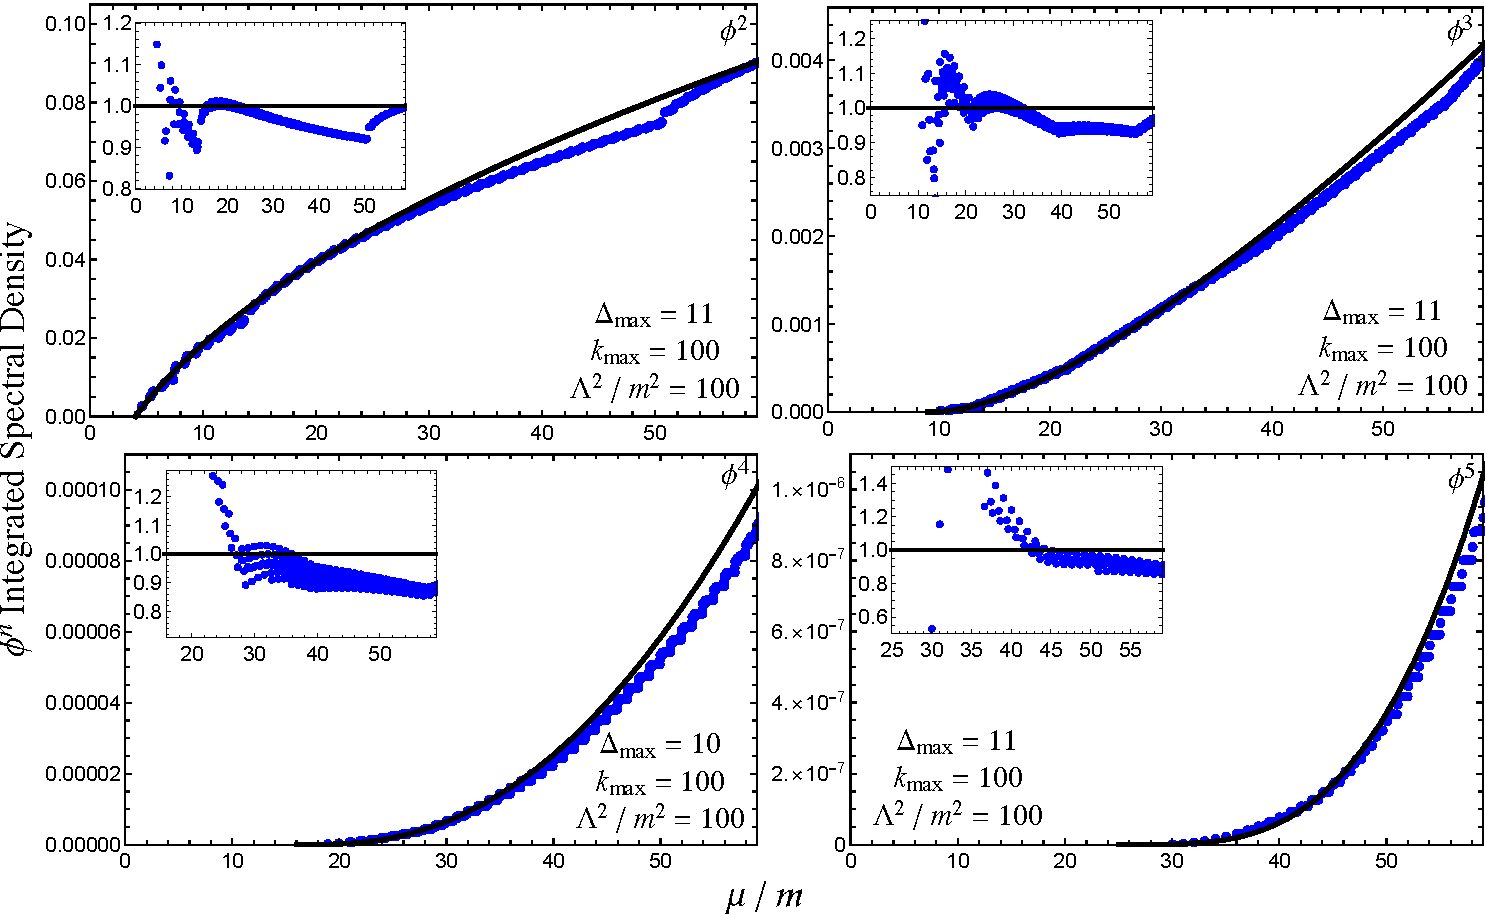
\includegraphics[width=\textwidth]{truncation_chapter/FreePhiN}
\caption{Integrated spectral densities for $\phi^2$ (upper left), $\phi^3$ (upper right), $\phi^4$ (lower left), and $\phi^5$ (lower right) in massive free field theory ($\lambda=0$), both the raw value (main plot) and normalized by the theoretical prediction (inset). The conformal truncation results (blue dots) for each plot are computed using the $\Dmax$ shown, with the corresponding number of $n$-particle basis states, and compared to the theoretical prediction (black curve).}
\label{fig:FreeDensities} 
\end{center}
\end{figure}

\begin{figure}[t!]
\begin{center}
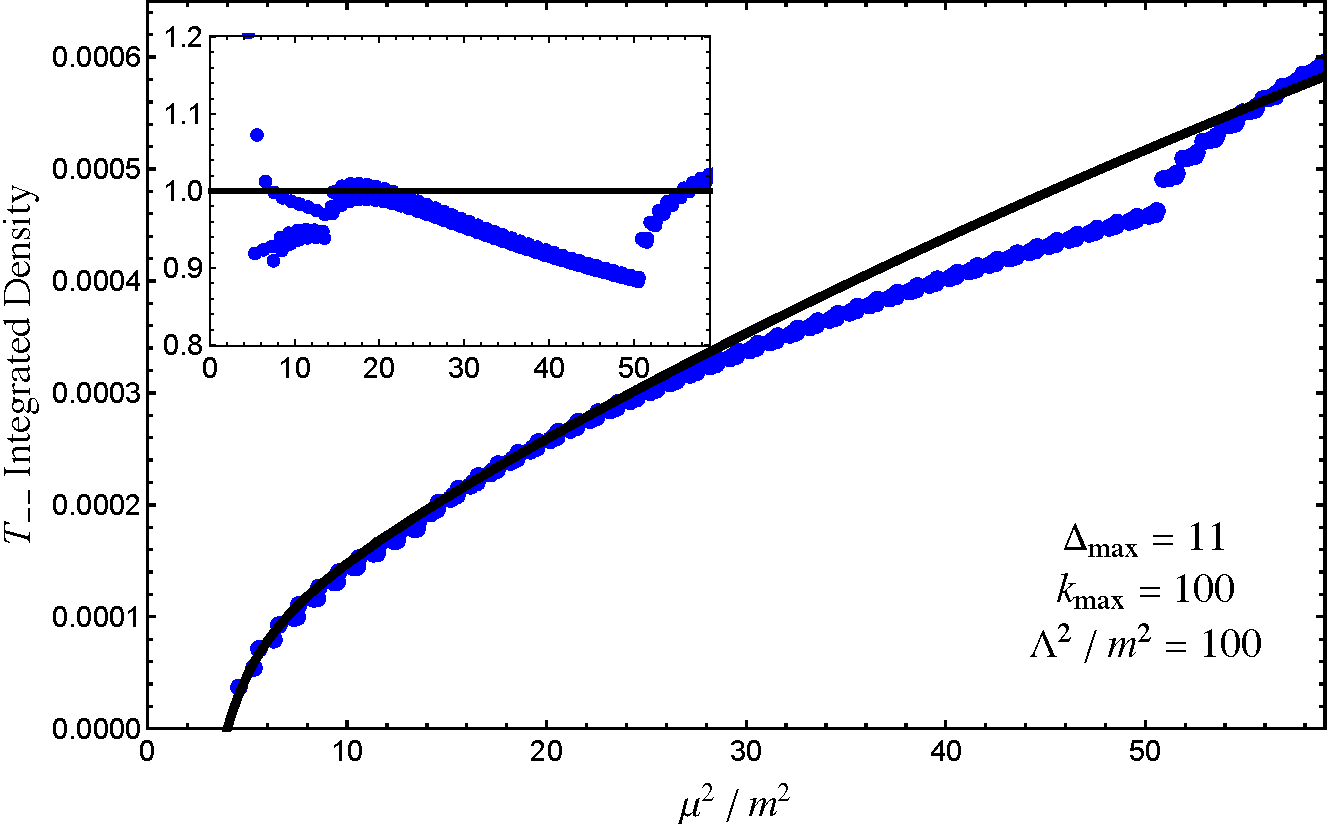
\includegraphics[width=\textwidth]{truncation_chapter/Tmm}
\caption{Integrated spectral densities for the stress tensor component $T_{--}$ in massive free field theory ($\lambda=0$), both the raw value (main plot) and normalized by the theoretical prediction (inset). The conformal truncation results (blue dots) for each plot are computed using the $\Dmax$ shown, with the corresponding number of $n$-particle basis states, and compared to the theoretical prediction (black curve).}
\label{fig:FreeDensitiesTmm} 
\end{center}
\end{figure}

\begin{figure}[t!]
\begin{center}
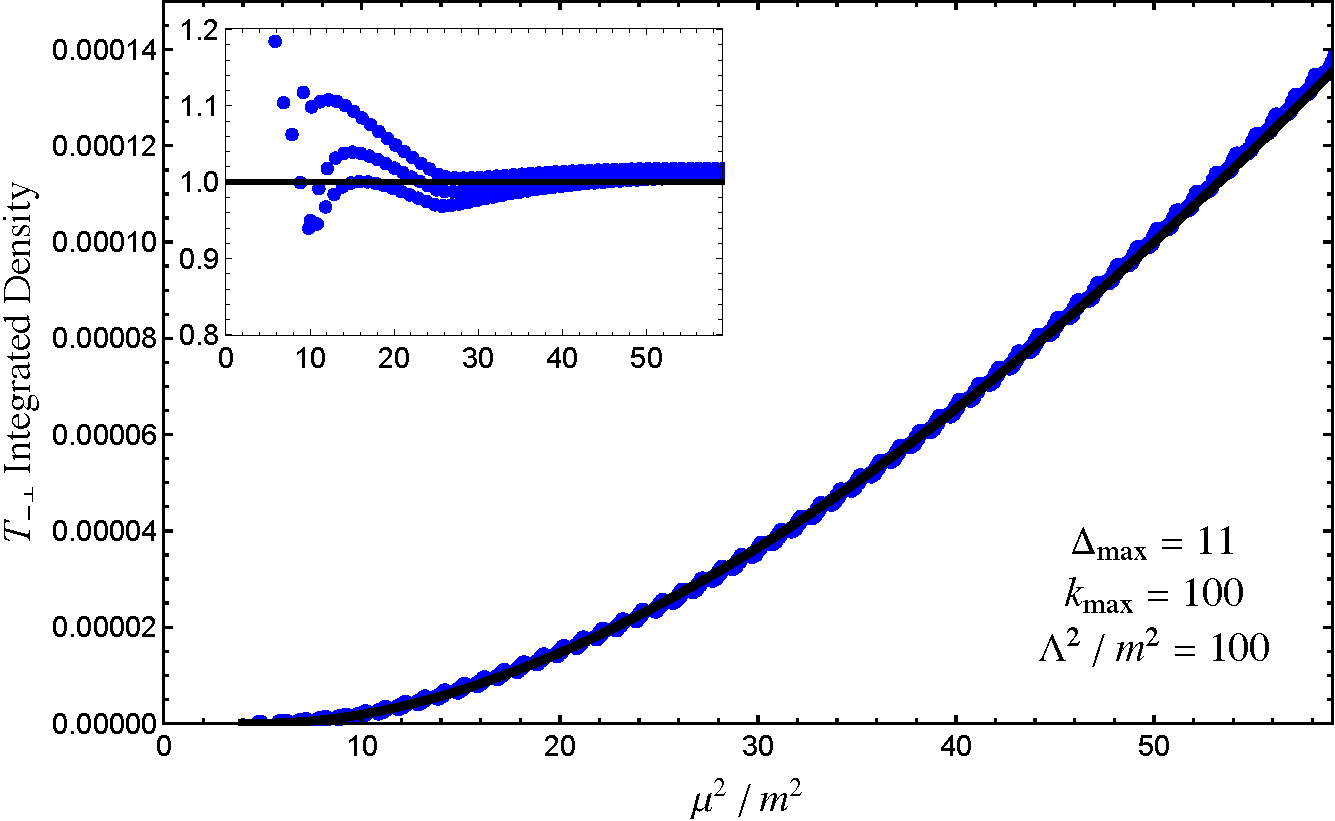
\includegraphics[width=\textwidth]{truncation_chapter/Tmp}
\caption{Integrated spectral densities for $T_{-\bot}$ in massive free field theory ($\lambda=0$), both the raw value (main plot) and normalized by the theoretical prediction (inset). The conformal truncation results (blue dots) for each plot are computed using the $\Dmax$ shown, with the corresponding number of $n$-particle basis states, and compared to the theoretical prediction (black curve).}
\label{fig:FreeDensitiesTmp} 
\end{center}
\end{figure}

\section{Discussion}
\label{sec:Discussion}

This project is still in the final debugging stages, but we believe it to be
numerically correct and are working on producing illustrative plots now. Figure
\ref{fig:hamiltonian} gives a visualization of the Hamiltonian created by the 
truncation methods of this chapter.

\begin{figure}
\centering
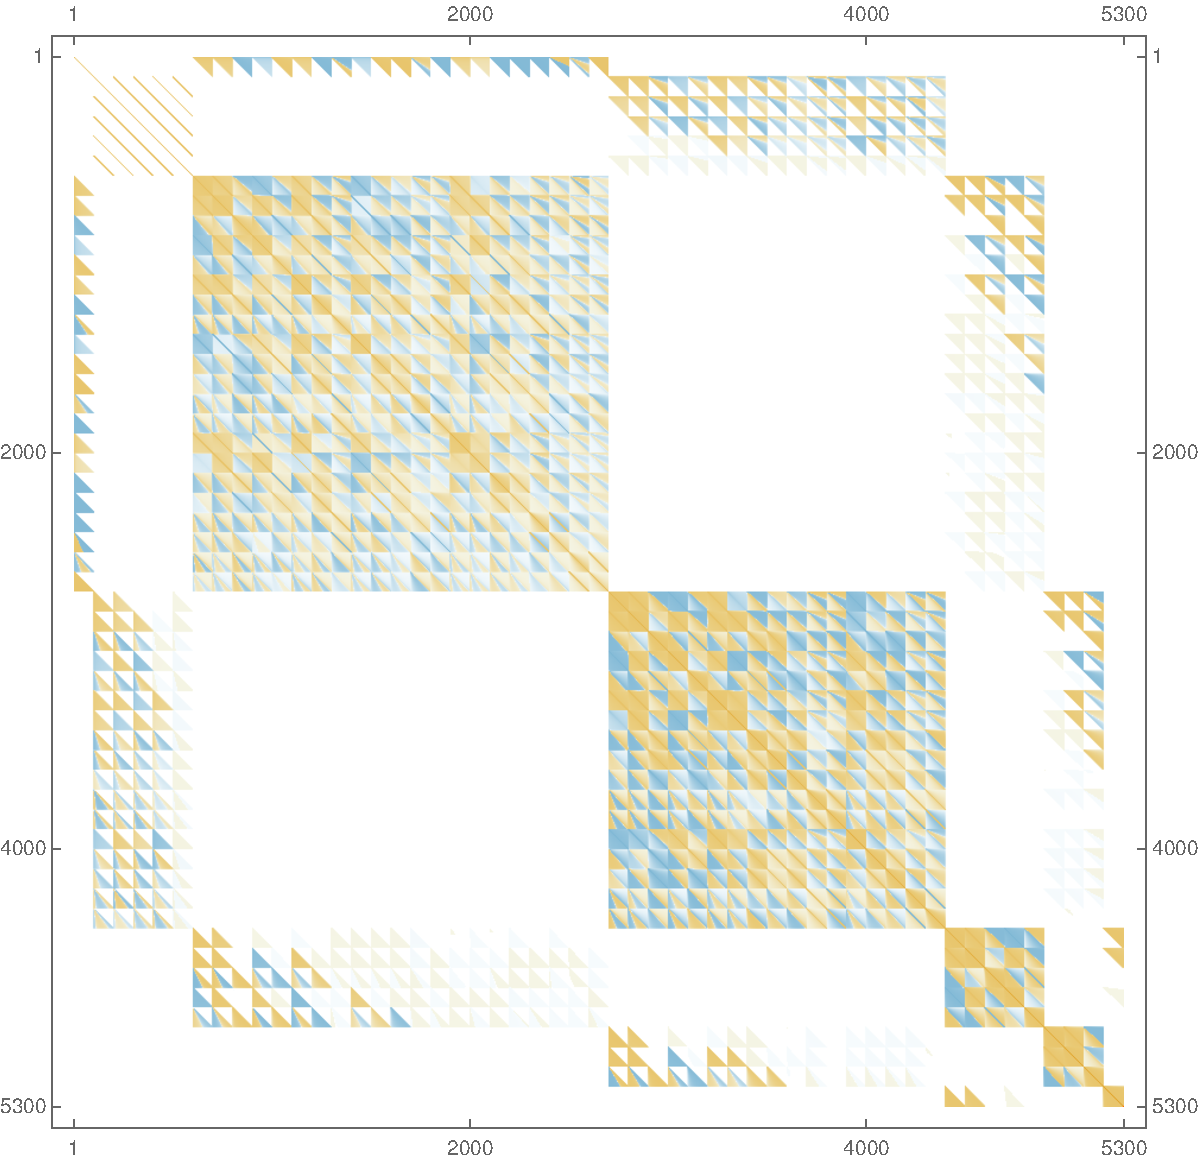
\includegraphics[width=0.9\textwidth]{truncation_chapter/hamiltonian}	
\caption[Visualization of truncated Hamiltonian]{This is the $P_\perp$-even 
    Hamiltonian produced with $\Delta_\mathrm{max} = 11$, 
    $k_\mathrm{max} = 100$, and $m^2 = \Lambda = \lambda = 1$. Warm colors are
    positive entries and cool colors are negative entries, with saturation 
    indicating the magnitude. The $n \to n+2$ entries outside of the diagonal
    blocks are jagged because these interactions are kinematically prohibited 
    when the low-$n$ state has more energy than the high-$n$ state, which is the
    half of the block closer to the diagonal.}
\label{fig:hamiltonian}
\end{figure}

In order to demonstrate the correctness of our truncation method, we can look at
the closing of the Ising model's mass gap as the strength of the deformation's 
coupling $\lambda$ is increased. This can be seen by finding the eigenvalues of 
the Hamiltonian and taking the lowest one -- this will be the mass of the 
1-particle state, which starts at a finite value and drops to 0 (along with the 
other states) as the mass gap closes. This is shown in figure \ref{fig:massgap}, 
and the observed behavior seems consistent with that seen in 2D and less 
comprehensive studies of 3D.

\begin{figure}
\centering
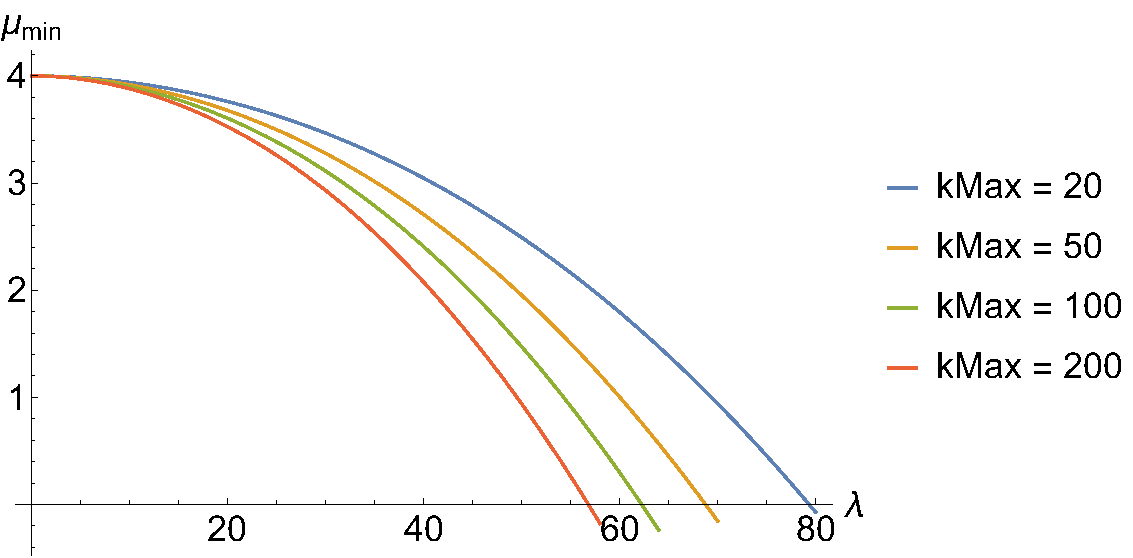
\includegraphics[width=0.9\textwidth]{truncation_chapter/massgap}	
\caption[Closing of the Ising model mass gap as a function of $\lambda$ for 
    different $k_\mathrm{max}$]{This shows the effective mass of the 
    single-particle state as a function of the interaction coupling $\lambda$. 
    Each of these is at $\Delta_\mathrm{max} = 8, m = 1, \Lambda = 20$, but 
    $k_\mathrm{max}$ is varied between 20 and 200, appearing to approach an 
    asymptotic `correct' value as $k_\mathrm{max} \to \infty$.} 
\label{fig:massgap}
\end{figure}


%%%%%%%%%%%%%%%%%%%%%%%%%%%%%%%%%%%%%%%%%%%%%%%%%%%%%%%%%%%%%%%%%%%%%%%%%%%%%
%%%%%%%%%%%%%%%%%%%%%%%%%%%%%%%%%%%%%%%%%%%%%%%%%%%%%%%%%%%%%%%%%%%%%%%%%%%%%
 

% \appendix
\begin{subappendices}

\section{Constructing the Basis of Dirichlet States}
\label{sec:ConstructingBasis}

By definition, the original basis of Casimir eigenstates consists of eigenstates 
of the CFT Hamiltonian. However, once we introduce a relevant mass deformation 
to the Hamiltonian 
\begin{equation}
    \delta P_+^{(m)} = \int \frac{d^2 p}{(2\pi)^2} a^\dagg_p a_p \frac{m^2}{2 p_-},
\end{equation} 
there are IR divergences associated with the mass matrix whenever any individual 
lightcone momentum of an $n$-particle eigenstate go to zero. If we regulate 
these divergences by introducing a small parameter $\epsilon$, the resultant 
mass spectrum contains two types of eigenstates: those that diverge as 
$\epsilon \to 0$ and those that remain finite. The states that diverge in this 
limit are lifted out of the spectrum, such that we can focus on the low-lying 
sector. The states that remain finite can be seen as a specific linear 
combination of Casimir eigenstates, a reshuffling of the original UV basis such 
that their eigenvalues are finite in the limit $\epsilon \to 0$. In practice, 
this reshuffling gives rise to a ``Dirichlet'' wavefunction 
$\tilde{F}_{\CO}^{(n)}(p)$ that is schematically the product of the lightcone 
momenta times a wavefunction which we denote $\bar{F}_{\CO}^{(n)}(p)$: 
\begin{equation}
    F_{\CO}^{(n)}(p) \to \tilde{F}_{\CO}^{(n)}(p) \sim p_{1-} p_{2-} \dotsb p_{n-} \bar{F}_{\CO}^{(n)}(p). \label{dirshuffle}
\end{equation} 
We will drop the $(n)$ superscript for brevity. 

It is important to note that the size of the Dirichlet basis is smaller than 
that of the original Casimir basis. While every Dirichlet state has this overall 
factor of $p_{1-} \dotsb p_{n-}$, we cannot obtain it from starting with the UV 
basis and simply tacking on the product of momenta. These states consist of 
\textit{specific} linear combinations of UV primaries that are orthogonal with 
respect to an inner product, and in the following section we outline how to 
numerically compute them.

\subsection{Two-Particle Example} Before we move onto the general case, we 
briefly review how the Dirichlet basis arises in a simple two-particle example. 
We will show how the addition of a mass deformation to the Hamiltonian 
reshuffles the basis, resulting in a divergent piece that is lifted out of the 
IR spectrum and a finite piece that is a physical state.

To see this, consider a truncated 2-particle basis consisting of the operators 
$\phi^2$ and $T_{--}$, where $T_{--}$ is given by\footnote{Up to a normalization 
constant that we will ignore as it is not important for this discussion.} 
\be 
    T_{--} = \phi \partial_-^2 \phi - 3(\partial_- \phi)^2. 
\ee 
In momentum space, we can express the wavefunction associated with $T_{--}$ as 
\begin{equation}
    \int d^3 x \, e^{i x \cdot P} \bra{\phi \partial_-^2 \phi (x) - 3 (\partial_- \phi)^2 (x)} p_1, p_2 \rangle = [6 p_{1-} p_{2-} -(p_1^2+p_2^2)] \times \delta(P-p_1-p_2), 
\end{equation} 
Let's first start with the simple example of the mass term matrix element 
between $\phi^2$. We find 
\begin{equation}
\begin{aligned}
    \langle {\phi^2; P'} |2P_- \delta P_+^{(m)} | {\phi^2, P} \rangle = &2P_- m^2 \int \frac{d^2 k_1 d^2 k_2}{(2\pi)^4 2 k_{1-} 2 k_{2-}} (2\pi)^3 \delta^3(k_1+k_2-P') \\
    &\times (2\pi)^3 \delta^3(k_1+k_2-P) \left(\frac{1}{k_{1-}} + \frac{1}{k_{2-}} \right).
\end{aligned}
\end{equation} 
Already, we can see how the divergence will arise. We see that when any of the 
$k_{i-} \to 0$, the integral above will exhibit a divergence which will need to 
be regulated. In fact, the delta functions cause the two integrals above to 
collapse to a single integral and introducing an $\epsilon$ regulator and 
performing that integral using the coordinate transformations in Appendix 
\ref{gencase}, we find 
\begin{equation}
    \langle \phi^2; P' | 2 P_- \delta P_+^{(m)} | \phi^2, P \rangle = 2P_-  (2\pi)^2 \delta(\vec{P}-\vec{P}') \frac{m^2}{\mu}\left(\frac{1}{\sqrt{P_- \epsilon}} + \mathcal{O}(\epsilon) \right),
\end{equation} 
where $P^2 =\mu^2$. As expected, this matrix element diverges as 
$1/\sqrt{\epsilon}$. Now, performing the same exercise for the other operator 
$T_{--}$, we find 
\begin{equation}
    \begin{aligned}
        \bra{T_{--}; P'} 2P_- \delta P_+^{(m)} \ket{ T_{--}; P} &= 2P_- (2\pi)^2 \delta^2(\vec{P}-\vec{P}') \frac{m^2}{\mu} \left( \frac{ P_-^{7/2}}{\sqrt{\epsilon}} + \mathcal{O}(\epsilon) \right).
    \end{aligned}
\end{equation} 
We can also similarly compute the matrix element between $T_{--}$ and $\phi^2$. 
Ignoring overall numerical factors and the $\mu$ dependence, we find that the 
divergent part of the matrix elements looks like 
\begin{equation}
    M^2 \sim \frac{1}{\sqrt{\epsilon}} \begin{pmatrix}
        P_-^{-1/2} & P_{-}^{3/2} \\
        P_{-}^{3/2} & P_{-}^{7/2}
    \end{pmatrix}
\end{equation} 
This matrix has two eigenvalues: 0 and one that diverges as $\epsilon \to 0$, 
which is $\sim \frac{1}{\sqrt{\epsilon}}$. If we look at the eigenvector 
corresponding to the former, we find that it is just a linear combination 
\begin{equation}
    \begin{pmatrix}
            P_-^2 & 1
    \end{pmatrix} = -P_-^2 \phi^2 + T_{--} = -(p_1+p_2)^2 \phi^2 + T_{--} = -\phi \partial_-^2 \phi - (\partial_- \phi)^2 + T_{--}.
\end{equation} 
We see that the $\phi \partial_-^2 \phi$ cancels against the same term in 
$T_{--}$, leaving just a term proportional to $(\partial_- \phi)^2$. The effect 
of the Dirichlet boundary condition is to therefore to \textit{reshuffle} the 
basis and remove the problematic piece in $T_{--}$. The reduced Dirichlet basis, 
which in this case consists of the single eigenstate corresponding to the 
operator $(\partial_- \phi)^2$, is the finite eigenstate, while the divergent 
piece is lifted out of the spectrum. In effect, the Dirichlet basis consists of 
reshuffling of the original basis such that the operators that remain have a 
product of momenta $p_{1-} p_{2-} \dotsb p_{n-}$ necessary to cancel against the 
IR divergence.

The purpose of this example was to show how the Dirichlet basis arises from the 
standard conformal primary basis once we deform by a mass term. We see that the 
size of the Dirichlet basis is smaller than that of the original basis (and this 
behavior will persist as we increase the size of the basis). In practice, one 
could construct the Dirichlet states by finding the finite linear combinations 
of eigenstates, which amounts to determining the kernel of the divergent part of 
the mass matrix. However, our approach will simply be to construct these states 
by demanding that every Dirichlet state has a product of momenta 
$p_{1-} p_{2-} \dotsb p_{n-}$ and using their associated inner product. We will 
describe this in the next section.

\subsection{General Case \label{gencase}} 
While the above method for constructing the Dirichlet basis can be generalized, 
in this work we will explicitly construct the basis of Dirichlet states from 
their associated inner product. This basis is identical to what is obtained by 
starting with Casimir eigenstates and demanding that they satisfy Dirichlet 
boundary conditions, but it is computationally more efficient to implement. We 
leave the details of our numerical algorithm to section \ref{sec:code}; below we 
will derive the Dirichlet inner product and explain the symmetrization procedure 
to obtain our final basis states.

Our Dirichlet states take the form as in eq. \eqref{eqn:finalbasisstates}, which 
we reproduce here: 
\begin{equation}
    \begin{aligned}
        | \mathcal{O};  \vec{P}, k \rangle = &\frac{1}{\sqrt{2\pi} P_-^{n + |\boldsymbol{\lambda}_-|} \Lambda^{\frac{n-5}{2} + |\boldsymbol{\lambda}_\bot|}}\int_0^{1} \frac{d\bar{\mu}^2}{\bar{\mu}^{\frac{n-3}{2} + |\boldsymbol{\lambda}_\bot|}} g_k(\bar{\mu}) \label{eqn:finalbasisstates}\\
        &\times \frac{1}{n!}\int \frac{d^2 p_1 \dotsb d^2 p_n}{(2\pi)^{2n} 2p_{1-} \dotsb 2p_{n-}} (2\pi)^3 \delta^3 \left( \sum_i p_i - P \right) \\
        &\times p_{1-} p_{2-} \dotsb p_{n-} \bar{F}_{\mathcal{O}}(p) | p_1, \dotsb, p_n \rangle,
    \end{aligned}
\end{equation} 
where we have substituted in the Dirichlet wavefunction in eq. 
(\ref{dirshuffle}). The inner product then takes the form 
\begin{equation}
    \begin{aligned}
        &\inner{\mathcal{O}';\vec{P}', k'}{\mathcal{O};\vec{P}, k} = \frac{2P_- (2\pi)^2 \delta^2(\vec{P}-\vec{P}')}{2^n n!} \frac{1}{2\pi P_-^{2n+ |\boldsymbol{\lambda}_-|+|\boldsymbol{\lambda}^{\prime}_\bot|} \Lambda^{n-5 + |\boldsymbol{\lambda}_\bot|+|\boldsymbol{\lambda}^{\prime}_-|}} \\
        &\times \int_0^{1} \frac{d\bar{\mu}^2}{\bar{\mu}^{\frac{n-3}{2} + |\boldsymbol{\lambda}_\bot|}} \int_0^{1} \frac{d\bar{\mu}^{\prime 2}}{\bar{\mu}^{\prime \frac{n-3}{2} + |\boldsymbol{\lambda}_\bot|}} g_k(\bar{\mu}^2) g_{k'}(\bar{\mu}^{\prime 2}) (2\pi) \delta(\bar{\mu}^2 - \bar{\mu}^{\prime 2}) \\
        &\times \int \frac{d^2 p_1 \dotsb d^2 p_n}{(2\pi)^{2n}} (2\pi)^3 \delta^3\left(\sum_i p_i - P \right)
        p_{1-} \dotsb p_{n-} \bar{F}_{\Ocal}(p) \bar{F}_{\Ocal'}(p).
    \end{aligned}
\end{equation} 
Using the equations of motion and the choice of our reference frame of 
$P_\bot = 0$, the set of delta functions can be recast as 
\begin{equation}
    \begin{aligned}
        \delta^3\left(\sum_i p_i - P \right) = \delta\left(\sum_i \frac{p_{i\bot}^2}{2p_{i-}} - \frac{\mu^2}{2P_-} \right)\delta\left(\sum_i p_{i-} - P_- \right)\delta\left(\sum_i p_{i\bot}\right).
    \end{aligned}
\end{equation} 
Here, it is useful to define dimensionless variables 
\begin{equation}
    x_i \equiv \frac{p_{i-}}{P_-},\quad\quad\quad\quad\quad\quad y_i \equiv \frac{p_{i\bot}}{\mu}, \label{dimlessvars}
\end{equation} 
so that the wavefunctions have a scaling set by 
\begin{equation}
    \tilde{F}_{\CO}(p) = \mu^{|\lamvec_\bot|} P_-^{n+|\lamvec_-|} x_1 \dotsb x_n \bar{F}_{\CO}(x,y),
\end{equation} 
where $|\lamvec_\bot|$ counts the number of $P_\bot$ derivatives while 
$|\lamvec_-|$ counts the number of $P_-$ derivatives in 
$\bar{F}_{\mathcal{O}}(p)$. These scaling factors cancel against the factors 
coming from the $\bar{\mu}$ integration measure. Since our weight functions are 
\textit{defined} to be orthonormal when integrated over $\mu^2$ with unit 
measure, the inner product factorizes into an orthogonal piece with respect to 
$k$ and $k'$ and a piece that depends on $\CO$ and $\CO'$: 
\begin{equation}
    \begin{aligned} 
        \inner{\mathcal{O}';\vec{P}', k'}{\mathcal{O};\vec{P}, k} = 2P_- (2\pi)^2 \delta^2 (\vec{P}-\vec{P}') \delta_{k k'} \mathcal{I}_{\mathcal{O'}\mathcal{O}}.
    \end{aligned}
\end{equation}

To determine $\mathcal{I}_{\mathcal{O'}\mathcal{O}}$, we can choose integration 
variables defined by 
\begin{equation}
    \begin{aligned}
        x_1 &= (1-z_1)(1-z_2)(1-z_3) \dotsb (1-z_{n-1}), \\
        x_2 &= \quad\quad\,\,\, z_1(1-z_2)(1-z_3) \dotsb (1-z_{n-1}), \\
        x_3 &= \quad\quad\,\,\, \quad\quad\quad\,\, z_2(1-z_3) \dotsb (1-z_{n-1}), \\
        &\vdots \quad\quad\quad\quad\quad\quad\quad\quad\quad \ddots \\
        x_n &= \quad\quad\quad\quad\quad\quad\quad\quad\quad\quad\quad\quad\quad\quad z_{n-1}, \label{xtrans}
    \end{aligned}
\end{equation} 
where the $z_i$ range from $[0, 1]$, and 
\begin{equation}
    \begin{aligned}
        y_1 &= -(y_2+ y_3 + \dotsb + y_n), \\
        y_2 &= \tilde{y}_1 \sqrt{z_1(1-z_1) \dotsb (1-z_{n-1})} - z_1(y_3 + \dotsb + y_n), \\
        y_3 &= \tilde{y}_2 \sqrt{z_2(1-z_2) \dotsb (1-z_{n-1})} - z_2(y_4 + \dotsb + y_n), \\
        & \, \, \, \vdots\\
        y_n &= \tilde{y}_{n-1} \sqrt{z_{n-1}(1-z_{n-1})}. \label{ytrans}
    \end{aligned}
\end{equation} 
In these variables, the original set of delta functions we had simply reduce to 
\begin{equation}
    \begin{aligned}
        \delta^3\left(\sum_i p_i - P \right) \to \frac{2}{\mu^3} \delta \left( \sum_i^{n-1} \tilde{y}_i^2 - 1 \right).
    \end{aligned}
\end{equation} 
Introducing angular variables for the remaining $\tilde{y}$ variables to 
implement this constraint 
\begin{equation}
    \begin{aligned}
        \tilde{y}_1 &= \sin \theta_1 \sin \theta_2 \dotsb \sin \theta_{n-2}, \\
        \tilde{y}_2 &= \cos \theta_1 \sin \theta_2 \dotsb \sin \theta_{n-2}, \\
        \tilde{y}_3 &= \cos \theta_2 \sin \theta_3 \dotsb \sin \theta_{n-2}, \\
        &\, \, \, \vdots \\
        \tilde{y}_{n-1} &= \cos \theta_{n-2}, \label{thetatrans}
    \end{aligned}
\end{equation} 
where $\theta_i \in [0, \pi]$ for $i = 1, \dots, n-3$ and 
$\theta_{n-2} \in [0, 2\pi]$, we find that the inner product becomes 
\begin{equation}
    \begin{aligned}
        \inner{\mathcal{O}';\vec{P}', k'}{\mathcal{O};\vec{P}, k} = 2P_- (2\pi)^2 \delta^2 (\vec{P}-\vec{P}') \delta_{k k'} \mathcal{I}_{\mathcal{O'}\mathcal{O}},
    \end{aligned}
\end{equation} 
with 
\begin{empheq}[box=\fbox]{align}
    \mathcal{I}_{\mathcal{O'}\mathcal{O}} =  \frac{1}{n! 2^n (2\pi)^{2n-3}} &\int dz_1 \dotsb dz_{n-1} \left( \prod_i z_i^{\frac{3}{2}} (1-z_i)^{\frac{5}{2}i-1} \right) \nonumber \\
    &\times \int d\theta_1 \dotsb d\theta_{n-2} \left( \prod_j \sin^{j-1} \theta_j \right) \bar{F}_{\Ocal}(z,\theta) \bar{F}_{\Ocal'}(z,\theta). \label{inner}
\end{empheq}

To obtain our final Dirichlet states, we tabulate a list of Dirichlet monomials 
at and below a given maximum Casimir eigenvalue $\mathcal{C}_{\textrm{max}}$. 
This set of monomials will be overcomplete, so in order to determine the 
complete orthonormal basis, we compute the Gram matrix using eq. (\ref{inner}) 
between different monomials. We then determine the final basis by performing a 
QR decomposition on the Gram matrix, the details of which we leave to Appendix 
\ref{sec:code}.

%%%%%%%%%%%%%%%%%%%%%%%%%%%%%%%%%%%%%%%%%%%%%%%%%%%%%%%%%%%%%%%%%%%%%%%%%%%%%
%%%%%%%%%%%%%%%%%%%%%%%%%%%%%%%%%%%%%%%%%%%%%%%%%%%%%%%%%%%%%%%%%%%%%%%%%%%%%
%%%%%%%%%%%%%%%%%%%%%%%%%%%%%%%%%%%%%%%%%%%%%%%%%%%%%%%%%%%%%%%%%%%%%%%%%%%%%


\section{Matrix Elements and Operator Overlaps}
\label{sec:MatrixElements}

In this section, we compute the matrix elements between the invariant mass $M^2$ 
and the Dircichlet basis states. The mass operator can be written in terms of 
momentum generators as 
\begin{equation}
    M^2 = 2P_+ P_- - P_\bot^2.
\end{equation} 
However, since the Hamiltonian deformations we will study do not break 
translational invariance, we can choose a reference frame where $P_-$ is fixed 
and $P_\bot = 0$. We can therefore compute the simpler matrix elements 
\begin{equation}
    \bra{\mathcal{O}'; \vec{P}', k'} M^2 \ket{\mathcal{O}; \vec{P}, k} = 2P_- \bra{\mathcal{O}'; \vec{P}', k'} P_+ \ket{\Ocal; \vec{P}, k}.
\end{equation} 
These matrix elements take the form 
\begin{equation}
    \begin{aligned}
        \bra{\mathcal{O}'; \vec{P}', k'} M^2 \ket{\mathcal{O}; \vec{P}, k} = 2P_- (2\pi)^2 \delta^2(\vec{P}- \vec{P}') {\Mcal}_{\mathcal{O},\mathcal{O}', \, k, k'}.
    \end{aligned}
\end{equation} 
We will suppress the overall kinematic factor and focus on the matrix elements 
$ \Mcal_{\mathcal{O},\mathcal{O}', \, k, k'}$ for the remainder of this section.

\subsection{Kinetic Term} 
We begin by computing the $M^2$ matrix elements in the original CFT. The CFT 
Hamiltonian can be expressed in terms of raising and lowering operators as 
\begin{equation}
    P_+^{(\textrm{CFT})} = \int \frac{d^2 p}{(2\pi)^2} a^\dagg_p a_p \frac{p_\bot^2}{2p_-}. \label{kineticP}
\end{equation} 
Note that this term preserves particle number, so that we consider sectors with 
differing particle number separately. As discussed in section 
\ref{sec:ConstructingBasis}, our Dirichlet states take the form 
\begin{equation}
    \begin{aligned}
        | \mathcal{O};  \vec{P}, k \rangle = &\frac{1}{\sqrt{2\pi} P_-^{n + |\boldsymbol{\lambda}_-|} \Lambda^{\frac{n-5}{2} + |\boldsymbol{\lambda}_\bot|}}\int_0^{1} \frac{d\bar{\mu}^2}{\bar{\mu}^{\frac{n-3}{2} + |\boldsymbol{\lambda}_\bot|}} g_k(\bar{\mu}) \label{eqn:finalbasisstates}\\
        &\times \frac{1}{n!}\int \frac{d^2 p_1 \dotsb d^2 p_n}{(2\pi)^{2n} 2p_{1-} \dotsb 2p_{n-}} (2\pi)^3 \delta^3 \left( \sum_i p_i - P \right) \\
        &\times p_{1-} p_{2-} \dotsb p_{n-} \bar{F}_{\mathcal{O}}(p) | p_1, \dotsb, p_n \rangle.
    \end{aligned}
\end{equation} 
Inserting eq. (\ref{kineticP}) in between two states and using the coordinate 
transformations in eqs. (\ref{xtrans}), (\ref{ytrans}), and (\ref{thetatrans}) 
we find that 
\begin{equation}
    \begin{aligned}
        \boxed{\Mcal^{(\textrm{CFT})}_{k, k'; \mathcal{O}, \mathcal{O}'} = \Lambda^2 \left( \frac{\mu_k^2 + \mu_{k-1}^2}{2} \right) \delta_{k, k'} \mathcal{I}_{ \mathcal{O}, \mathcal{O}'}.}
    \end{aligned}
\end{equation}

\subsection{Mass Term} 
The first deformation we consider to the UV Hamiltonian is the mass term, which 
results in a correction 
\begin{equation}
    \begin{aligned}
        \delta P_+^{(m)} &= \int \frac{d^2 p}{(2\pi)^2} a^\dagg_p a_p \frac{m^2}{2p_-}.
    \end{aligned}
\end{equation} 
Like the kinetic term, this term preserves particle number. We can use the same 
coordinate transformations as in the inner product and kinetic terms to arrive 
at 
\begin{empheq}[box=\fbox]{align}
    \Mcal^{(m)}_{k, k'; \Ocal, \Ocal'} = &\delta_{k , k'} \frac{m^2}{(n-1)! 2^n (2\pi)^{2n-3}} \int dz_1 \dotsb dz_{n-1} \left( \prod_i z_i^{\frac{3}{2}} (1-z_i)^{\frac{5}{2}i-1}  \right) \\
    &\times \left( \frac{1}{z_{n-1}} \right) \nonumber
    \int d\theta_1 \dotsb d\theta_{n-2} \left( \prod_j \sin^{j-1} \theta_j \right) \bar{F}_{\Ocal}(z,\theta) \bar{F}_{\Ocal'}(z,\theta). 
\end{empheq}

\subsection{Quartic Interaction} 
We now move onto the more nontrivial deformation of a quartic interaction to the 
Hamiltonian, which gives rise to a Hamiltonian correction of the form 
\begin{equation}
    \begin{aligned}
        \delta P_+^{(\lambda)} = \frac{\lambda}{24} \int \frac{d^2p d^2 q d^2 k}{(2\pi)^6 \sqrt{8 p_- q_- k_-}} \left( \frac{4 a^\dagg_p a^\dagg_q a^\dagg_k a_{p+q+k}}{\sqrt{2(p_- + q_- + k_-)}} + \textrm{ h.c. } + \frac{6 a^\dagg_p a^\dagg_q a_k a_{p+q-k}}{\sqrt{2(p_- + q_- - k_-)}} \right). \label{quarticdef}
    \end{aligned}
\end{equation} 
This deformation contains two types of terms, one that changes particle number 
and one that preserves it. We will refer to the former, which corresponds to the 
first two terms in eq. \eqref{quarticdef}, as the $n$-to-$n+2$ interaction since 
it changes particle number by two. We will call the latter type of term in eq. 
\eqref{quarticdef} the $n$-to-$n$ interaction.

Unlike the kinetic and mass terms, the interaction terms give rise to matrix 
elements that depend separately on both $\mu$ and $\mu'$. In other words, the 
discretization integrals over $\mu$ and $\mu'$ do not collapse into one simple 
integral, but instead depend on $\mu$ and $\mu'$ through the ratio 
\begin{equation}
    \boxed{\alpha \equiv \frac{\mu}{\mu'} .}
\end{equation} 
For this reason, we will introduce the useful notation 
\begin{equation}
    \begin{aligned}
        &\bra{\Ocal'; \vec{P}', k'} \delta M^2 \ket{\Ocal; \vec{P}, k} = 2P_- (2\pi)^2 \delta^2(\vec{P}- \vec{P}') \\
        &\times  \frac{\lambda \Lambda}{2\pi} \frac{1}{P_-^{2n+ |\boldsymbol{\lambda}_-|+|\boldsymbol{\lambda}^{\prime}_\bot|} \Lambda^{n-5 + |\boldsymbol{\lambda}_\bot|+|\boldsymbol{\lambda}^{\prime}_-|}}\int_0^{1} \frac{d\bar{\mu}^2}{\bar{\mu}^{\frac{n-3}{2} + |\boldsymbol{\lambda}_\bot|}} \int_0^{1} \frac{d\bar{\mu}^{\prime 2}}{\bar{\mu}^{\prime \frac{n-3}{2} + |\boldsymbol{\lambda}_\bot|}}  g_k(\bar{\mu}^2) g_{k'}(\bar{\mu}^{\prime 2}) \Mcal_{\Ocal \Ocal'}(\alpha).
    \end{aligned}
\end{equation} 
The computation of $\Mcal_{\Ocal \Ocal'}(\alpha)$ for the interaction terms will 
be the main focus of the following two sections. 

\subsubsection{$n$-to-$n+2$ Interaction} 
Let's first consider the $n$-to-$n+2$ interaction, which gives rise to the 
following matrix element between an $n$ particle state and an $n+2$ particle 
state: 
\begin{equation}
    \begin{aligned}
        \Mcal^{(n\textrm{-to-}n+2)}_{\Ocal \Ocal'}(\alpha) &= \frac{\lambda}{6(n-1)!} \int \frac{d^2 p_1 \dotsb d^2 p_n}{(2\pi)^{2n} 2p_{1-} \dotsb 2p_{n-}} (2\pi)^3 \delta^3 \left(\sum_i p_i - P \right) p_{1-} \dotsb p_{n-} \bar{F}_{\Ocal}(p) \\
        &\times \int \frac{d^2p_1' \dotsb d^2p_{n+2}'}{(2\pi)^{2n+4} 2p_{1-}' \dotsb 2p'_{n+2-}} (2\pi)^3 \delta^3\left(\sum_i p'_i - P' \right) p'_{1-} \dotsb p'_{n+2-} \bar{F}_{\Ocal'}(p') \\
        &\times 2p_{2-} (2\pi)^2 \delta^2(p_2 - p'_4) \dotsb 2 p_{n-} (2\pi)^2 \delta^2 (p_n - p'_{n+2}).
    \end{aligned}
\end{equation} 
It is useful to switch to the dimensionless variables defined in eq. 
(\ref{dimlessvars}) separately for the both the primed and unprimed variables. 
That is, we take eq. \eqref{xtrans}-\eqref{ytrans} for the unprimed variables 
and 
\begin{equation}
    \begin{aligned}
        x_1' &= (1-z'_1)(1-z'_2)(1-z'_3) \dotsb (1-z'_{n+1}), \\
        x_2' &= \quad\quad\,\,\, z'_1(1-z'_2)(1-z'_3) \dotsb (1-z'_{n+1}), \\
        x_3' &= \quad\quad\,\,\, \quad\quad\quad\,\, z'_2(1-z_3') \dotsb (1-z_{n+1}'), \\
        &\vdots \quad\quad\quad\quad\quad\quad\quad\quad\quad \ddots \\
        x_{n+2}' &= \quad\quad\quad\quad\quad\quad\quad\quad\quad\quad\quad\quad\quad\quad z_{n+1}' \label{xtransprimed}
    \end{aligned}
\end{equation} 
for the primed coordinates and analogously for eq. \eqref{ytrans}. We then find 
\begin{equation}
    \begin{aligned}
        &\Mcal^{(n\textrm{-to-}n+2)}_{\Ocal \Ocal'}(\alpha) = \frac{\lambda n \sqrt{(n+1)(n+2)}}{24 \pi} \frac{1}{\mu'} \alpha^{\frac{n-3}{2}} \int dz_1 \dotsb dz_{n-1}   d\tilde{y}_1 \dotsb d\tilde{y}_{n-1}  \\
        &\times \left( \prod_{i=1}^{n-1} z_i^{\frac{3}{2}} (1-z_i)^{\frac{5}{2}i+1} \right) \delta\left(\sum_i^{n-1} \tilde{y}^2_{n-1} -1  \right) \bar{F}_{\Ocal}(z,\tilde{y}) \\
        &\times \int dz'_1 dz'_2  d\tilde{y}'_1 d\tilde{y}_2'\, {z'_1}^{\frac{1}{2}} (1-z'_1)^{\frac{1}{2}} {z'_2}^{\frac{1}{2}} (1-z'_2)^2 \\
        &\times \delta\left(\tilde{y}_1^{\prime 2} + \tilde{y}_2^{\prime 2} + \alpha^2 \sum_{i=1}^{n-1} \tilde{y}_i^2 - 1 \right) \bar{F}_{\Ocal'}(z', \tilde{y},\tilde{y}').
    \end{aligned}
\end{equation} 
The first delta function constrains the $n-1$ $\tilde{y}$'s, which correspond to 
the variables of the ``spectator'' particles, to a sphere of radius 1. The other 
delta function for the interacting particles constrains $\tilde{y}'$ to a sphere 
of radius $1-\alpha^2$, which constrains $\alpha \le 1$. Physically, this is due 
to the fact that the $n$-to-$n+2$ interactions can only increase the kinetic 
energy due to the creation of two additional particles. Parameterizing these two 
spheres with angular variables for the spectators and interacting particles we 
obtain 
\begin{empheq}[box=\fbox]{align}
    &\Mcal^{(n\textrm{-to-}n+2)}_{\Ocal \Ocal'}(\alpha) = \frac{1}{(n-1)! 3 \pi^{2n} 2^{3n+4}} \frac{1}{\mu'} \alpha^{\frac{n-3}{2}}  \nonumber \\
    &\times \int dz_1 \dotsb dz_{n-1} dz'_1 dz'_2   \left( \prod_{i=1}^{n-1} z_i^{\frac{3}{2}} (1-z_i)^{\frac{5}{2}i+1} \right) {z'_1}^{\frac{1}{2}} (1-z'_1)^{\frac{1}{2}} {z'_2}^{\frac{1}{2}} (1-z'_2)^2 \nonumber \\
    &\times \int d\theta_1 \dotsb d\theta_{n-2} d\theta' \left(\prod_j \sin^{j-1} \theta_j \right) \bar{F}_{\Ocal}(z,\theta) \bar{F}_{\Ocal}(z',\theta',\theta,\alpha).
\end{empheq}

\subsubsection{$n$-to-$n$ Interaction} 
Finally, we turn to the $n$-to-$n$ part of the quartic interaction. It takes the 
form 
\begin{equation}
    \begin{aligned}
        \Mcal_{\Ocal \Ocal'}^{(n-\textrm{to}-n)}(\alpha) = &\frac{\lambda n(n-1)}{4} \frac{1}{n!} \int \frac{d^2p_1 \dotsb d^2 p_n}{(2\pi)^{2n} 2p_{1-} \dotsb 2p_{n-}} (2\pi)^3 \delta^3\left(\sum_i p_i - P \right) \\
        &\times p_{1-} \dotsb p_{n-} \bar{F}_{\Ocal}(p) \int \frac{d^2 p'_1 \dotsb d^2 p'_n}{(2\pi)^{2n} 2p'_{1-} \dotsb 2p'_{n-}} \\
        &\times (2\pi)^3 \delta^3\left(\sum_i p'_i - P' \right) p'_{1-} \dotsb p'_{n-} \bar{F}_{\Ocal}(p') \\
        &\times 2p_{3-}(2\pi)^2 \delta^2(p_3 - p_3') \dotsb 2p_{n-} (2\pi)^2 \delta^2(p_n -p'_n).
    \end{aligned}
\end{equation} 
Performing the coordinate transforms in eqs. \eqref{xtrans}-\eqref{ytrans} for 
both the primed and unprimed coordinates, we find 
\begin{equation}
    \begin{aligned}
        \Mcal_{\Ocal \Ocal'}^{(n-\textrm{to}-n)}(\alpha) =& \frac{\lambda n(n-1) \alpha^{\frac{n-3}{2}}}{16 \pi \mu'} \int dz_1  d\tilde{y}_1 dz'_1 d\tilde{y}'_1 \sqrt{z_1 (1-z_1) z'_1 (1-z'_1)} \\
        &\times \delta\left(\sum_i \tilde{y}_i^2 - 1 \right) \delta\left({\tilde{y}_1}^{\prime 2} +  \alpha^2 \sum_{i =2}\tilde{y}_i^2  -1\right) \\
        &\times \int dz_2 \dotsb dz_{n-1} d\tilde{y}_2 \dotsb d\tilde{y}_{n-1} \left( \prod_{i>1} z_i^{\frac{3}{2}} (1-z_i)^{\frac{5i-3}{2}} \right) \\
        &\times F_{\Ocal}(z,\tilde{y}) F_{\Ocal}(z',\tilde{y}').
    \end{aligned}
\end{equation} 
We can use the delta functions to perform the integration over the $\tilde{y}$ 
coordinates of the interacting particles. Note that they impose the constraints 
\begin{equation}
    \tilde{y}_1 = \pm\sqrt{1-r^2}, \quad\quad\quad\quad\quad \tilde{y}_1^{\prime} = \pm \sqrt{ 1 - \alpha^2 r^2},
\end{equation} 
where 
\begin{equation}
    r^2 \equiv \tilde{y}_2^2 - \tilde{y}_3^2 \dotsb - \tilde{y}_{n-1}^2.
\end{equation} 
Note that when $\alpha =1$, the two constraints coincide, and the range of 
integration $r$ is taken to be between $[0,1]$. Similarly, when $\alpha < 1 $, 
the reality condition on $\tilde{y}_1$ requires $r \in [0,1]$, which 
automatically satisfies the constraint on $\tilde{y}'_1$. However, when 
$\alpha > 1$, the reality condition on $\tilde{y}'_1$ provides a stronger 
constraint and requires $r \in [0, \alpha^{-1} ]$.

Defining spherical coordinates for the remaining spectators 
\begin{equation}
    \begin{aligned}
        \tilde{y}_2 &= r \sin \theta_1 \sin \theta_2 \dotsb \sin \theta_{n-3}, \\
        \tilde{y}_3 &= r \cos \theta_1 \sin \theta_2 \dotsb \sin \theta_{n-3}, \\
        \tilde{y}_4 &= r \cos \theta_2 \sin \theta_3 \dotsb \sin \theta_{n-3}, \\
        &\, \, \, \vdots \\
        \tilde{y}_{n-1} &= r \cos \theta_{n-3},
    \end{aligned}
\end{equation} 
and defining 
\begin{equation}
    \bar{F}_{\Ocal \pm} \equiv \bar{F}_{\Ocal}(\tilde{y}_1 = \pm \sqrt{1-r^2}),\quad\quad\quad\quad \bar{F}_{\Ocal' \pm} \equiv \bar{F}_{\Ocal'}(\tilde{y}_1 = \pm \sqrt{1-\alpha^2 r^2}),
\end{equation} 
the matrix element can be summarized as 
\begin{empheq}[box=\fbox]{align}
    &\Mcal^{(n\textrm{-to-}n)}_{\Ocal \Ocal'}(\alpha) = \frac{1}{(n-2)! \pi^{2n-2} 2^{3n+2}} \frac{1}{\mu'} \alpha^{\frac{n-3}{2}}  \nonumber \\
    &\times \int dz_1 \dotsb dz_{n-1} dz'_1 \sqrt{z_1(1-z_1)z'_1(1-z'_1)} \left(\prod_{i > 1} z_i^{\frac{3}{2}} (1-z_i)^{\frac{5i-3}{2}} \right) \nonumber \\
    &\times \int_0^{\min \left(1,\alpha^{-1} \right)} dr \int d\theta_1 \dotsb d\theta_{n-3} \left( \prod_j \sin^{j-1} \theta_j \right) \frac{r^{n-3}}{\sqrt{(1-r^2)(1-\alpha^2 r^2)}} \nonumber \\
    &\times \left(\sum_{\pm} \bar{F}_{\Ocal}(z,r,\theta) \right)\left(\sum_{\pm} \bar{F}_{\Ocal'}(z,\alpha r, \theta) \right).
\end{empheq}

%%%%%%%%%%%%%%%%%%%%%%%%%%%%%%%%%%%%%%%%%%%%%%%%%%%%%%%%%%%%%%%%%%%%%%%%%%%%%
%%%%%%%%%%%%%%%%%%%%%%%%%%%%%%%%%%%%%%%%%%%%%%%%%%%%%%%%%%%%%%%%%%%%%%%%%%%%%
%%%%%%%%%%%%%%%%%%%%%%%%%%%%%%%%%%%%%%%%%%%%%%%%%%%%%%%%%%%%%%%%%%%%%%%%%%%%%


\section{Details of Code and Algorithms}
\label{sec:code}

Broadly speaking, the goal of the program is to reduce as many computations as
possible to pure linear algebra operations. This allows us both to avoid a great
deal of repeated work and to take advantage of established libraries for linear
algebra. So in order to do this, we need a basis for all relevant operators and
we need to express the quantities of interest as vectors and matrices on this
basis.

Our computation begins with a naive list of all Dirichlet monomials having total 
scaling dimension below some cutoff $\Delta$. We intend to use this as a basis
for all states below the cutoff, but since it's vastly overcomplete, we must 
first eliminate all of the redundant monomials, the first step of which is to 
compute the Gram matrix containing the inner products of all of the monomials in 
the naive list with all of the others. Before computing the Gram matrix, we 
normalize the input monomials so that it's easier to distinguish floating point 
epsilons from inner products which just happen to be small, and we also separate
the states with an even number of $P_\perp$ derivatives from those with an odd
number: the former are always orthogonal to the latter, and their matrix 
elements with each other are always zero, so we can treat both cases separately.
Since matrix algorithms generally have complexity of roughly $O(N^3)$, any
simplification which breaks the overall matrix up into invariant subspaces is 
tremendously advantageous.

With the Gram matrix in hand, there are a number of ways to produce an 
orthogonal basis from the overcomplete one, the simplest of them being a QR
decomposition. However, the QR decomposition of a rank-deficient matrix is not
unique, and the Gram matrix is rank-deficient due to the basis being 
overcomplete. This is a mixed blessing: while it means that off-the-shelf QR
decomposition functions will often yield a correct but non-useful basis, it also
means that we have a lot of freedom to arrange to produce the most convenient
basis possible.

Our implementation uses the Modified Gram-Schmidt Algorithm 
\cite{Code:ModGramSchmidt}, feeding in monomials one at a time starting with the
monomials with the most evenly distributed powers of $P_-$ and $P_\perp$. This
produces a basis where the fewest possible monomials are used, which is 
desirable because it's $~O(N^2)$ easier to compute matrix elements between 
single monomials than between arbitrary superpositions of them. The evenly 
distributed exponents on the monomials means that each individual monomial will
have fewer unique permutations, again simplifying the computation of the matrix
elements.

Note that the Gram-Schmidt process produces exponentially compounding roundoff
errors in the coefficients of the output vectors because each coefficient 
depends on all of the ones before it. Because of this problem, we found that we
had to use 128-bit precision floating point numbers to keep epsilons from 
growing to sizes comparable to the actual answers; if one were to increase total 
scaling dimension beyond what we attempted, one would likely need to increase
the precision further, which could quickly create performance bottlenecks.

Having finished Gram-Schmidt and obtained a basis of orthonormal states, the
next step is to actually compute the matrix elements between these states. All
of the matrix elements are bilinear in the two states' reduced wavefunctions
$\bar F$, which themselves are sums of permutations of ordered monomials. This
suggests a second layer of linear algebra structure: we can represent the 
orthonormal basis states as vectors on the (non-orthonormal) space of ordered
monomials which appear in them. 

We refer to this latter space as the `minimal basis' and write the orthonormal 
polynomial basis as a matrix $P$ whose columns each represent one of the 
polynomials, with entry $(i,j)$ giving the contribution of minimal basis 
monomial $i$ to orthonormal polynomial $j$. Now, to produce matrix elements 
between the orthonormal basis polynomials, we can simply compute the matrix 
elements $M_{ij}$ between minimal basis monomials and transform them to 
$P^T M P$, producing exactly the desired matrix. Note that $M$ and $P$ are
precisely the same size in our implementation, thanks to our choice of
orthogonalization of the naive basis -- if we had not deliberately selected one 
which used as few individual monomials as possible, $M$ could have been several 
times larger.

The matrix $M$ is properly a 4th-order tensor relating the $k$th $\mu^2$ 
partition of monomial $m$ to the $k'$th $\mu^2$ partition of monomial $m'$, i.e.
we're computing the entries $M_{mkm'k'}$. For computation simplicity, however,
we actually treat this as a matrix: if there are $N_m$ minimal basis monomials
and $N_k$ $\mu^2$ partitions, then $M$ is an $N_m N_k \times N_m N_k$ matrix
where each pair of monomials has its own $N_k \times N_k$ block. 

We compute $M$ block by block, first getting an overall factor $a$ by doing all 
of the integrals not involving $\mu^2$, then computing a discretization matrix 
$D$ and multiplying it by $a$. The entry $D_{ij}$ contains the integral of all
$\mu^2$ factors across the appropriate window:
\begin{equation}
    D_{ij} = \int_{i/N_k}^{(i+1)/N_k} d\mu^2 \int_{j/N_k}^{(j+1)/N_k} d\mu'^2
             f(\mu^2, \mu'^2).
    \label{eq:discMatrix}
\end{equation}
For the kinetic and mass matrices, $f(\mu^2, \mu'^2)$ is just proportional to
$\delta(\mu^2 - \mu'^2)$, while for the interaction matrices it's close to a 
polynomial in $\mu^2/\mu'^2$. We memoized each discretization matrix in a hash
table keyed by $f(\mu^2, \mu'^2)$, so a matrix element calculation can be 
represented with the following pseudocode:
\begin{verbatim}
for each unique permutation of m and m':
  do integrals to get {numerical factor a} and {list of which f appear}
  for each f which appears:
    answer += a * D(f)
return answer * degeneracy
\end{verbatim}
where the degeneracy is the number of permutations which are indistinguishable
from a given unique permutation; which is of course the same for every unique 
permutation so it becomes an overall factor. Note that if the integrals in 
\eqref{eq:discMatrix} can be done analytically, it's possible to program in the
answers as a function of a given set of input exponents. This is fantastically
faster and more precise than a numerical integration, being able to quickly get
10 or 15 decimal digits of precision while the latter struggles to get 5.

Once all of the minimal basis matrices $M$ have been computed, everything else
is just standard matrix algebra. In particular, the Hamiltonian is just
\begin{equation}
    \sum_i P^T M_i P,
\end{equation}
summed over the kinetic, mass, and interaction terms. Interesting quantities
like eigenvalues can then be computed using ordinary matrix libraries; one might
think that some special care is required to take advantage of various properties
of the matrix, for instance the fact that it is ``block sparse'' in that the
block of $n$-particle states is coupled only to itself and the blocks of $n-2$-
and $n+2$-particle states. However, because the bulk of the states lie in the
middle of the particle number range, this actually includes quite a large 
proportion of the possible pairs, and in fact upon inspection one sees that the
matrix is about half full at $\Delta_\mathrm{max} = 10$. If 
$\Delta_\mathrm{max}$ were increased further, the matrix would become 
increasingly sparse (technically block sparse), but we do not expect that it 
would be worth considering sparse methods such as the Lanczos algorithm until 
$\Delta_\mathrm{max} = 15$ or higher.

Using the double linear algebra formulation and aggressive memoization of all
the repeated work we could find, we were able to produce finished matrices up to
$\Delta_\mathrm{max} = 10, k_\mathrm{max} = 100$ on an ordinary desktop computer 
in around two minutes. We believe that we will be able to solve everything up to 
around $\Delta_\mathrm{max} = 15$ before the resulting matrices become too large 
to deal with; this is our main obstacle, since $k_\mathrm{max}$ must be kept
high to maintain good convergence. If $k_\mathrm{max}$ is kept at 100, the final
matrices become unwieldy once more than about 100 orthogonal states are 
introduced, which happens at around $\Delta_\mathrm{max} = 15$.

%%%%%%%%%%%%%%%%%%%%%%%%%%%%%%%%%%%%%%%%%%%%%%%%%%%%%%%%%%%%%%%%%%%%%%%%%%%%%
%%%%%%%%%%%%%%%%%%%%%%%%%%%%%%%%%%%%%%%%%%%%%%%%%%%%%%%%%%%%%%%%%%%%%%%%%%%%%


\end{subappendices}
